
%(BEGIN_QUESTION)
% Copyright 2006, Tony R. Kuphaldt, released under the Creative Commons Attribution License (v 1.0)
% This means you may do almost anything with this work of mine, so long as you give me proper credit

It is often possible to configure a valve positioner in such a way to reverse the action (signal-to-open or signal-to-close) of a control valve.  One reason to do this is to create one-half of a split range, where the other valve acts in the opposite (either complementary or exclusive) manner.  Consider the following control valve, whose positioner has been configured to respond in ``reverse:''

$$\includegraphics[width=15.5cm]{i01399x01.eps}$$

While this may be possible, it might not be the best thing to do from a perspective of fail-safe.  Explain why the fail-safe mode of this valve may be compromised with such a positioner calibration.  Then, explain what the {\it best} way would be to reverse the action of the valve.

\vskip 20pt \vbox{\hrule \hbox{\strut \vrule{} {\bf Suggestions for Socratic discussion} \vrule} \hrule}

\begin{itemize}
\item{} A powerful problem-solving technique is performing a {\it thought experiment} where you mentally simulate the response of a system to some imagined set of conditions.  Describe a useful ``thought experiment'' for this system, and how the results of that thought experiment are helpful to answering the question.
\item{} Identify a practical reverse-acting range for a control valve, and an application where it might be used.
\end{itemize}

\underbar{file i01399}
%(END_QUESTION)





%(BEGIN_ANSWER)

The failure mode of this valve due to loss of supply air pressure to the positioner will not be the same as the failure mode due to loss of air pressure from the I/P or due to loss of DC current to the I/P.
 
%(END_ANSWER)





%(BEGIN_NOTES)

As configured in the illustration:

\begin{itemize}
\item{} Failed air supply to positioner = {\it valve closes}
\item{} Failed air supply to I/P = {\it valve opens}
\item{} Failed current signal to I/P = {\it valve opens}
\end{itemize}

\vskip 10pt

A better way to reverse this valve's response is to reverse the actuator and make the positioner direct-acting, thus changing the valve from air-to-open to air-to-close.  This way, the failure mode will be consistent (valve closes) regardless of where air pressure (or current signal) is lost.

%INDEX% Final Control Elements, valve: positioner

%(END_NOTES)


